\chapter{\altGerEng{Verwandte Arbeiten}{Related Work}}

Many related works have been performed previously to eliminate the necessity of external power or batteries for biasing power or further processing of the signal received. This chapter of the thesis paper will discuss approaches that have already been carried out in the past in designing the transmitter and receiver, opto-channel modeling, \ac{EH}, data modulation and demodulation, and, in general, wireless light-data communications.

The paper \cite{fan2017circuit} proposes simultaneous optical data reception and \ac{EH} using a photovoltaic cell. Figure \ref{fig:2.1} illustrates the circuit used in the paper. The circuit has two branches: one for \ac{EH} and another for communication. Similarly, in the paper \cite{liu2016visible}, a solar cell is used to directly convert optical signals into electrical signals, requiring no external power supply. Paper \cite{mahmoud2022design} and \cite{wang2015design} provided a similar model circuit for \ac{SLIPT}, shown in Figure \ref{fig:2.2}.

\begin{figure}
    \centering
    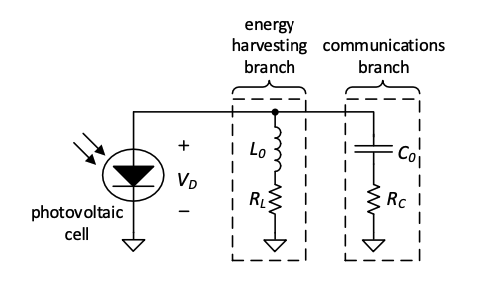
\includegraphics[width=0.75\linewidth]{fig/Schematic diagram of the circuit consists of an energy harvesting branch and a communications branch.png}
    \caption{Schematic diagram of the circuit consists of an \ac{EH} branch and
a communications branch. \cite{fan2017circuit}}
    \label{fig:2.1}
\end{figure}

\begin{figure}
    \centering
    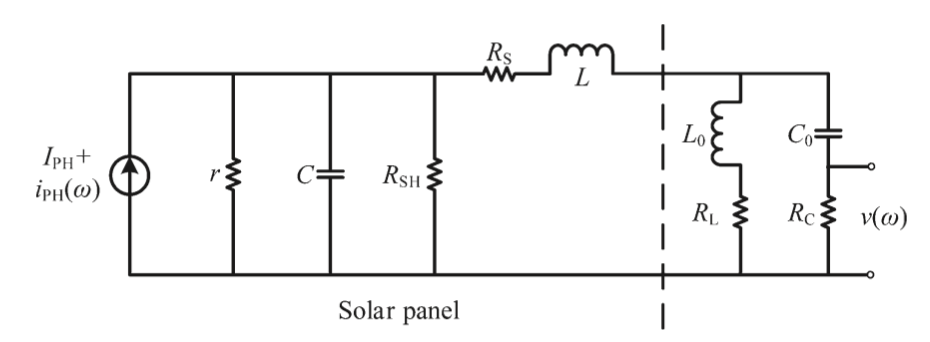
\includegraphics[width=0.75\linewidth]{fig/Solar cell model: an equivalent circuit in a configuration for synchronous energy harvesting and data communication..png}
    \caption{An equivalent circuit in a configuration for synchronous energy harvesting and data communication. \cite{mahmoud2022design}\cite{wang2015design}}
    \label{fig:2.2}
\end{figure}

The paper \cite{liu2016visible} proposes using a pre-distortion function to enhance solar cell receivers' response significantly. Experimental results show that the response of the solar cell receiver is greatly improved, with the original 2-kHz detection bandwidth being improved by 250 times. This allows for the reception of a 500-kbit/s \ac{VLC} signal at a transmission distance of 1 meter. 

In contrast, the paper \cite{Shin:16} presented a self-reverse-bias receiver circuit designed to enhance communication and \ac{EH} performance. The proposed system achieved a transmission rate of 17.05 Mbps with a bit error rate of 1.1x \( 10^{-3}\) and improved solar energy conversion efficiency. In addition, the 3-dB bandwidth increases from 90 to 120 kHz when reverse bias is increased from 0 to 30 V. Figure \ref{fig:2.3} shows the proposed receiver circuit for using a solar panel as a receiver for communication with simultaneous \ac{EH}.

\begin{figure}
    \centering
    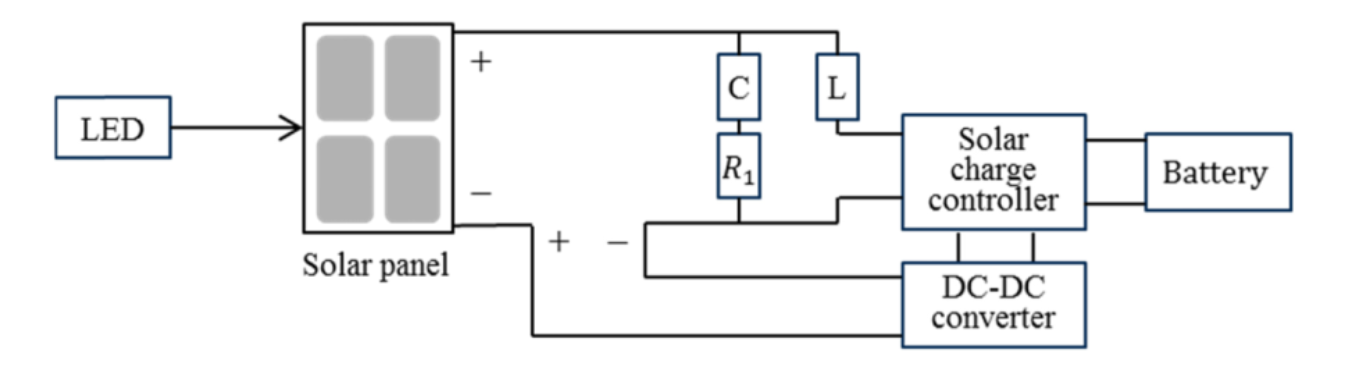
\includegraphics[width=0.75\linewidth]{fig/olar panel based on self-reverse-biased receiver circuit for simultaneous energy harvesting and communication.png}
    \caption{Solar panel based on self-reverse-biased receiver circuit for simultaneous energy harvesting and communication.\cite{Shin:16}}
    \label{fig:2.3}
\end{figure}

Paper \cite{dondi2007photovoltaic} discusses the \ac{MPPT} techniques adopted in its design and describes the actual implementation of a \ac{PV} harvester over a wide range of irradiance conditions. This paper also presents a PSpice numerical model for small photovoltaic sources, which is beneficial for designing integrated photovoltaic systems. The model is specifically designed for energy scavenger circuits used in sensor nodes\cite{dondi2007photovoltaic}.

The paper \cite{wang2022high} introduces a GaAs/AlGaAs-based modified uni-traveling-carrier \ac{PD} for simultaneous energy and data collection, which operates under forward bias. This method exhibits high-speed data transmission of 11.9 GHz and power conversion efficiency of 38.5\%.

The paper \cite{pan2017secure} discusses a secure hybrid \ac{VLC} and \ac{RF} system with visible light communication capabilities and contains a Light \ac{EH} model for \ac{PD}s. The authors examine a hybrid system with a legitimate receiver equipped with \ac{PD} for data communication and light \ac{EH}.

The paper \cite{fong2012integrated} proposes a system that integrates a \ac{PD} array, a DC-DC converter with \ac{MPPT}, and several components, including a sensor, an \ac{ADC}, and a \ac{DSP} in a single chip. The \ac{PD} used in this paper are custom-made \cite{fong2012integrated} with gratings, work in \ac{PV} mode, and have diffractive storage capacitance. 

The paper \cite{de2024reconfigurable} built an \ac{SLIPT}-based system made of an array of \ac{PD}s, which are arranged in a three-by-three configuration. These \ac{PD}s can switch between Photoconductive and Photovoltaic modes with a command from the internal \ac{MCU}. Prototype from this paper can receive data at 85 Mbps and harvest energy not only for self-power but also power additional sensors\cite{de2024reconfigurable}. 

The authors of the paper \cite{ma2019simultaneous} propose a simultaneous wireless information and power transfer (SWIPT) that has both the \ac{PD} and the solar panel, utilizing the \ac{PD} for information reception and the solar panel for \ac{EH}. Figure \ref{fig:2.4} shows the system block diagram of its transmission side. Figure \ref{fig:2.5} shows the adopted power-splitting technique to obtain separated signals at the receiver.

\begin{figure}
    \centering
    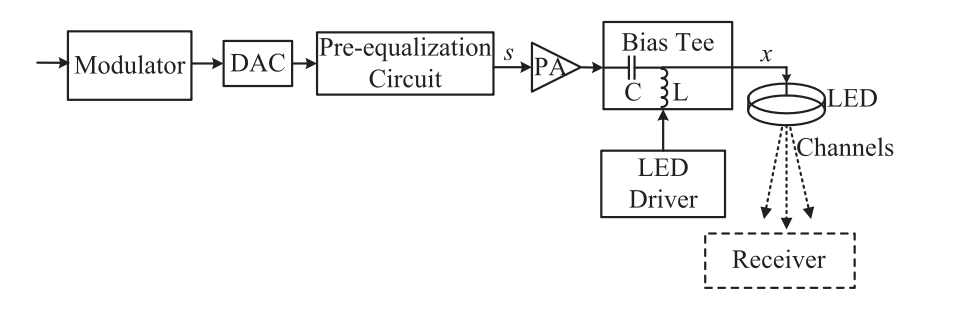
\includegraphics[width=0.5\linewidth]{fig/Schematic diagram of the SLIPT VLC system..png}
    \caption{Schematic diagram of the \ac{SLIPT} \ac{VLC} system transmitter. \cite{ma2019simultaneous}}
    \label{fig:2.4}
\end{figure}

\begin{figure}
    \centering
    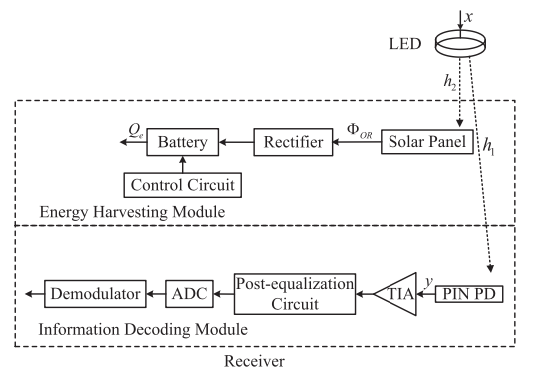
\includegraphics[width=0.5\linewidth]{fig/Structure combining information receiving and energy harvesting.png}
    \caption{Structure combining information receiving and \ac{EH}.\cite{ma2019simultaneous}}
    \label{fig:2.5}
\end{figure}

According to the paper \cite{haydaroglu2014optical}, LEDs can also be used for \ac{EH} and data reception. This paper describes a compact microsystem that integrates a single LED die serving as a power supply and data transmitter, with an \ac{ASIC} die and a storage capacitor.
A multi-LED and multi-user \ac{SLIPT} \ac{VLC} network is shown in the paper \cite{ma2019simultaneous}. The benefits of \ac{MIMO} are also showcased by the paper \cite{de2024reconfigurable} using an array of \ac{PD}s. For example, each \ac{PD} can decode from a specific source and will increase overall data communication.


The baseline Lambertian Optical channel Model is discussed in detail in the paper \cite{mossaad2015visible} along with the \ac{EH} Model, \ac{SLIPT} strategies, and Optimization. The authors of the paper \cite{diamantoulakis2018simultaneous}  also aim to optimize the balance between harvested energy, achievable rate, and \ac{SINR}.

This paper \cite{ding2024performance} explores the fundamental performance characteristics of non-Lambertian optical beams using \ac{SLIPT}. Additionally, it estimates the impact of beam azimuth rotation on improving the \ac{EH} efficiency of the \ac{SLIPT} system.
